%\flushleft
In this section we describe the overall goal of the project, the internal organisation and work distribution of our group, and our activities during the Blast-off of the project.  \\

\subsection{Goal of the Software}

In this subsection we describe the goal of the Test Data Analyser (TDA). The TDA is developed for medatixx GmbH \& Co. KG, a company that develops software for medical practices. TDA is an application to help software developers and testers at medatixx to analyse test data of their software. Purpose, advantage, and measurement are the three parts of which the goal of TDA is made of. \\
\ \\
{\large\textbf{Purpose}}\\ 

During the development of their software, medatixx uses a sequence of builds, i.e. (pre-)release versions of the software. To ensure the quality of their product, each build is tested via a number of unit tests which are defined and executed on the classes of the corresponding build. The collection of these unit tests, their classes and the build they belong to, and their results is called a test run. TDA shall support the analysis of these test runs to help medatixx to discover builds with classes that are problematic to test. \\ 
To do so, TDA shall extract the necessary information from the test run XML files provided by medatixx, analyse the information in different ways including the usesage of the Apriori algorithm and visualise the results of the information analysis. \\ 
\ \\

{\large\textbf{Advantage}}\\ 
The TDA provides new and more detailed information on the tests of different builds. It highlights the classes with the highest failure percentage of a specific test run. It shows the evolution of a class by visualising its failure percentages over multiple test runs. By using the Apriori algorithm it shows possible associations between different classes. It offers an easy method to compare the tests of a specific class in different test runs. \\ 
With the additional information the TDA is making available for testers at medatixx, they get new insight into their testing methodology and the overall test quality is improved. \\
\ \\

{\large\textbf{Measurement}}\\ 
Due to the easily accessible information on test runs and the discovered associations between classes, the resolution of failed classes and their corresponding unit tests shall be accelerated by at least 30 \%. 

%TODO: Find better solution for table
\newpage
\subsection{Organisation of the Group}
\begin{longtable}{|p{0.2\textwidth}||p{0.35\textwidth}|p{0.35\textwidth}|p{0.1\textwidth}|}
  \hline
  
  
    Name & Responsibilities & Principal Artefacts & Work Time\\
    \hline
    \hline
    Frank Keßler & Identify user stories & User story cards & 5 \\
    \hline
    Frank Keßler & StAX Parser & Methods for parsing & 3 \\ 
    \hline
    Frank Keßler & Preparing paper prototype & Paper prototype & 6 \\ 
    \hline
    Frank Keßler & Documenting Sprint 1 planning meeting & Sprint 1 planning wiki & 3 \\
    \hline
    Frank Keßler & Documenting Sprint 1 review meeting & Sprint 1 review wiki & 3 \\
	\hline
	Frank Keßler & Documenting Sprint 1 Daily scrum 3 & Sprint 1 Daily Scrum 3 wiki & 3 \\
	\hline
    Frank Keßler & Documenting Sprint 4 daily scrum 2 & Sprint 4 daily scrum 2 wiki & 3 \\
	\hline
	Frank Keßler & Documenting Sprint 5 planning meeting & Sprint 5 planning meeting wiki & 3 \\
	\hline
	Frank Keßler & Documenting Sprint 5 mid-sprint review meeting & Sprint 5 mid-sprint review meeting wiki & 3 \\
	\hline
	Frank Keßler & Documenting Sprint 5 Daily scrum 3 & Sprint 5 Daily Scrum 3 wiki & 3 \\
	\hline
    Frank Keßler & Low level architecture & Low level architechture diagram & 10 \\ 
    \hline
    Frank Keßler & data structure & classes in database package & 20 \\ 
    \hline 
    Frank Keßler & Loading correct testrun in Table from treeview & Corresponding methods & 6 \\ 
    \hline
    Frank Keßler & Sidebar classes view & Corresponding methods & 11 \\ 
    \hline
    Frank Keßler & Line-Chart view & Chart - Tab with corresponding classes & 12 \\ 
    \hline
    Frank Keßler & Comparison view & corresponding methods & 6\\
    \hline
    Frank Keßler & Loading correct class in chart & Corresponding methods & 8 \\ 
    \hline
    Frank Keßler & Changed classlist to a tree based structure & Treenode.java & 10 \\ 
    \hline
    Frank Keßler & Refactoring of whole project & Refactored project & 8 \\ 
    \hline
    Frank Keßler & Author of chapter 2 & Chapter in project report & 10 \\ 
    \hline
    \hline 
    \textbf{Total \newline Frank Keßler} & & & \textbf{total 136}   \\
    \hline
    \hline
    Andreas & Identify user stories & User story cards & 5 \\
    \hline
    Andreas & Create stakeholder map & stakeholder map & 3 \\ 
    \hline
    Andreas & StAXParser & Methods for parsing & 10 \\ 
    \hline
    Andreas & Preparing paper prototype & Paper prototype & 6 \\
    \hline
    Andreas & Create high level architecture diagram & High level architechture diagram & 4 \\ 
    \hline
    Andreas & Documenting Sprint 2 & Sprint 2 wiki & 3 \\ 
    \hline 
    Andreas & Directory browser in GUI & Corresponding methods & 3 \\ 
    \hline
    Andreas & Tree view and handling for imported test runs & Corresponding methods & 11 \\ 
    \hline
    Andreas & Testing of classes in package logic without Parser, Analyzer & JUnit tests & 12 \\ 
    \hline 
    Andreas & Create use case diagram & use case diagram & 10 \\ 
    \hline
    Andreas & Exception handling in StAXParser & Corresponding methods & 2 \\ 
    \hline
    Andreas & Documentation of Model & Javadoc in Model & 2 \\ 
    \hline
    Andreas & Documentation of Logic classes & Javadoc in Logic & 8 \\ 
    \hline
    Andreas & Author of chapter 1 & Chapter in project report & 10 \\ 
    \hline
    Andreas & Author of chapter 4.1 & Chapter in project report & 3 \\ 
    \hline
    Andreas & Author of chapter 4.2 & Chapter in project report & 12 \\
    \hline 
    Andreas & Author of chapter 4.3 & Chapter in project report & 10 \\ 
    \hline
    \hline 
    \textbf{Total \newline Andreas} & & & \textbf{total 114}   \\
    \hline
    \hline
    Jan Martin & Identify new user stories & User story cards & 4 \\
    \hline
    Jan Martin & Create use case diagram & use case diagram & 4 \\ 
    \hline
    Jan Martin & Improve UML diagram & Diagram in UMLLab & 6 \\ 
    \hline  
    Jan Martin & Implement TestData class & TestData class and connected classes & 4 \\ 
    \hline  
    Jan Martin & Implement File Browser & Corresponding methods & 4 \\ 
    \hline
    Jan Martin & Planning/Implementation of MVC architecture & Corresponding methods & 6 \\ 
    \hline  
    Jan Martin & Implementation on Navigation Menu & Corresponding methods & 2 \\ 
    \hline  
    Jan Martin & Product Backlog & Sprint <=2 Product Backlog in wiki & 2 \\ 
    \hline  
    Jan Martin & Implementation of Class Table with Simon & Class Table in GUI & 6 \\ 
    \hline  
    Jan Martin & Documenting Sprint 3 & Sprint 3 minutes & 2 \\ 
    \hline 
    Jan Martin & Implement TestRun Summary & TestRun Totals class & 2 \\ 
    \hline  
    Jan Martin & refactor TestRun totals & Corresponding methods & 6 \\ 
    \hline  
    Jan Martin & Research Apriori & Gained Team Knowledge & 5 \\ 
    \hline  
    Jan Martin & Implement Apriori & First Version of Apriori Analyzer classes & 21 \\ 
    \hline  
    Jan Martin & Class Distance Calculation & Corresponding methods & 6 \\ 
    \hline  
    Jan Martin & Documentation of Controller and Table classes & Javadoc in controller & 6 \\ 
    \hline    
    Jan Martin & Exception Handling/refactor of Controller class & Corresponding Methods & 2 \\ 
    \hline  
    Jan Martin & Controller Tests & none, aborted & 1 \\ 
    \hline  
    Jan Martin & Author of chapter 4.4 & Chapter in project report & 4 \\ 
    \hline
    Jan Martin & Co-Author of chapter 4.5 & Chapter in project report & 2 \\
    \hline 
    Jan Martin & Author of chapter 4.6 & Chapter in project report & 3 \\ 
    \hline
    Jan Martin & Author of chapter 5 & Chapter in project report & 10 \\ 
    \hline
    \hline 
    \textbf{Total \newline Jan} & & & \textbf{total}   \\
    \hline
    \hline
    Simon Meyer & Identify user stories & User story cards & 4 \\
    \hline
    Simon Meyer& Create SMART tasks for user stories & Tasks & 4 \\
    \hline
    Simon Meyer& Create and digitalize high-level architecture diagram & High-level architechture diagram & 3 \\ 
    \hline
    Simon Meyer& Create, improve and digitalize stakeholder map & Stakeholder map & 2 \\ 
    \hline
    Simon Meyer& Sketch and improve activity diagrams & Activity diagrams & 5 \\ 
    \hline
    Simon Meyer& Create use case diagram & Use case diagram & 2 \\ 
    \hline
    Simon Meyer& Prepare paper prototypes and other mockups for GUI elements and additional scenario & Paper prototype & 7 \\
    \hline
    Simon Meyer& Implement TestedClass logic and relation to other classes & Corresponding methods & 7 \\ 
    \hline
    Simon Meyer& Prepare resources, presentation and questions for meetings with client or scrum master & Prepare meetings & 5 \\ 
    \hline
    Simon Meyer& Develop and refine GUI/view for all visible elements & GUI & 40 \\ 
    \hline
    Simon Meyer& Implement underlying logic of TDAcomparisonView & Corresponding methods & 13 \\ 
    \hline
    Simon Meyer& Documenting Sprint 1 & Sprint 1 wiki & 3 \\ 
    \hline 
    Simon Meyer& Documenting Sprint 4 & Sprint 4 wiki & 2 \\ 
    \hline 
    Simon Meyer& Author of chapter 6 & Chapter in project report & 15 \\ 
    \hline
    \hline 
    \textbf{Total \newline Simon} & & & \textbf{total 112}   \\
    \hline
    \hline
  \caption{Distribution of work}
\end{longtable}


\subsection{Project Blast-off}

The Project Blast-off is the most important activity to decide whether or not to go ahead with a project. It is used to gather information on the project and make sure that it is viable and well founded. \\ 
Before we defined our goal for the project, we agreed that every member of our group should read and understand the project brief until our first official meeting. In our first meeting we collectively went through the requirements and every single described scenario. After making sure we were all on the same page and understood the content, we defined our goal of the whole project as described in subsection 1.1. \\ 
We continued by going through it again and highlighting epics and first user stories. In further cycles we worked on detailing them and lastly started on finding adequate tasks for the now written cards. Those tasks were not yet assigned to individual persons, as we still wanted to have the option to allocate them according to one’s time and knowledge on the described topic later on. Soon first challenges arose when it came down to connecting tasks with one adequate user story. It appears that some tasks are used for many user stories, because they describe core functionalities and therefore have to be implemented in order to make the rest working. Then again, sometimes it was just difficult to assign a specific task to a user story at all, because it described a mandatory functionality that just wasn’t covered by any adequate user story and creating one seemed not to be possible. We decided to discuss our concerns in the first meeting with the client.\\ 
During further discussion we identified the stakeholders of the project as shown in the stakeholder map in figure \ref{StakeMap}. \\ 

\newpage

\begin{figure}[h]
\begin{center}
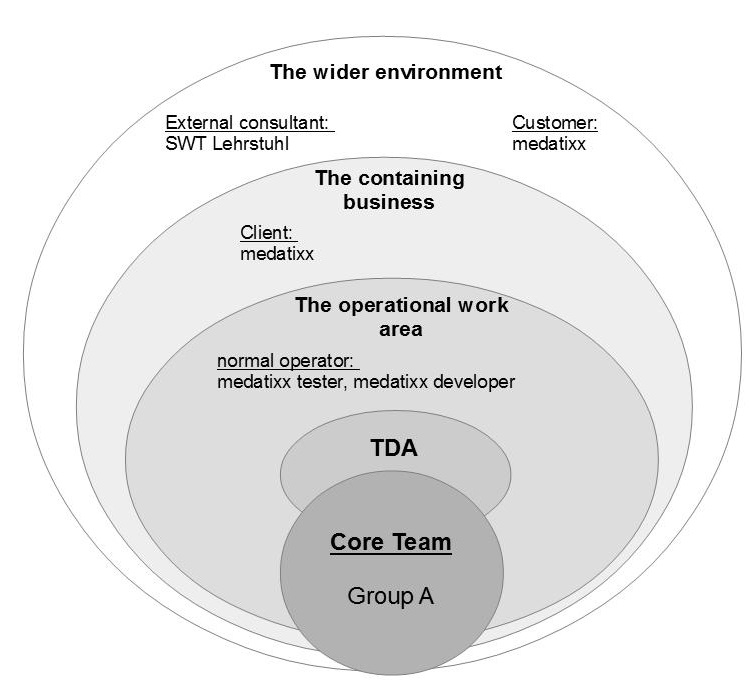
\includegraphics[scale=0.5]{pics/StakeMap2.jpg}
\caption{Stakeholder map}
\label{StakeMap}
\end{center}
\end{figure}

As you can see in figure \ref{StakeMap} medatixx GmbH \& Co. KG is listed as customer and client, since they use the TDA as an inhouse application. The typical users or normal operators of TDA are software testers and developers at medatixx. \\ 
In the next step we thought about the boundaries of our system, i.e. the scope of the work. As shown in figure \ref{Scope}, the TDA only has one indirect interface to adjacent systems. That interface is used by medatixx to provide the XML files from which TDA extracts the necessary information. We visualised this connection in the following context diagram. \\

\newpage

\begin{figure}[h]
\begin{center}
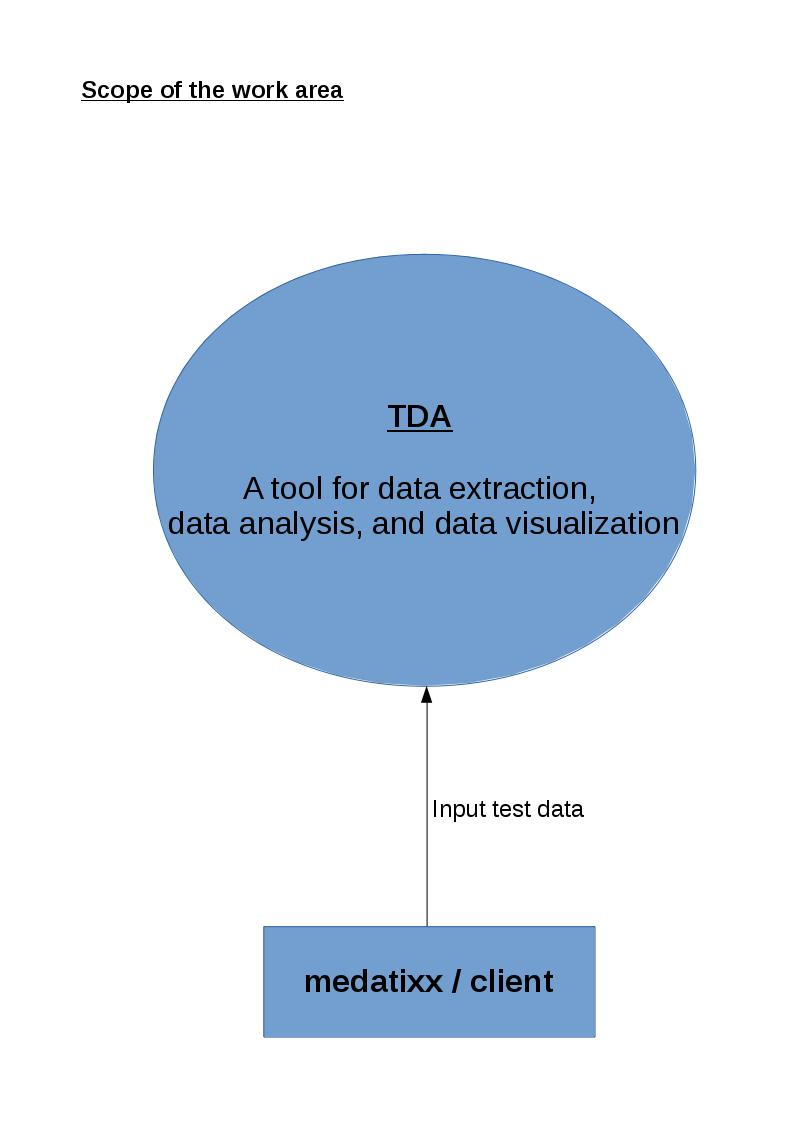
\includegraphics[scale=0.2]{pics/Scope_of_Work_Context_Diagram_v2.jpg}
\caption{Context diagram} 
\label{Scope}
\end{center}
\end{figure}

After we defined the scope of work of the TDA we discussed which architecture and design patterns we could use for our system. Also first ideas for specific classes and interfaces arose. Gladly, all of us had already visited the DSG-AJP-B course in previous semesters and so we could all contribute equally to the discussion without too much additional explanation of any named techniques. Since we have to deliver a GUI application in Java, we decided on a standard model-view-controller pattern. The corresponding high level architecture diagram is shown below in figure \ref{HLA}. \\ 

\newpage

\begin{figure}[h]
\begin{center}
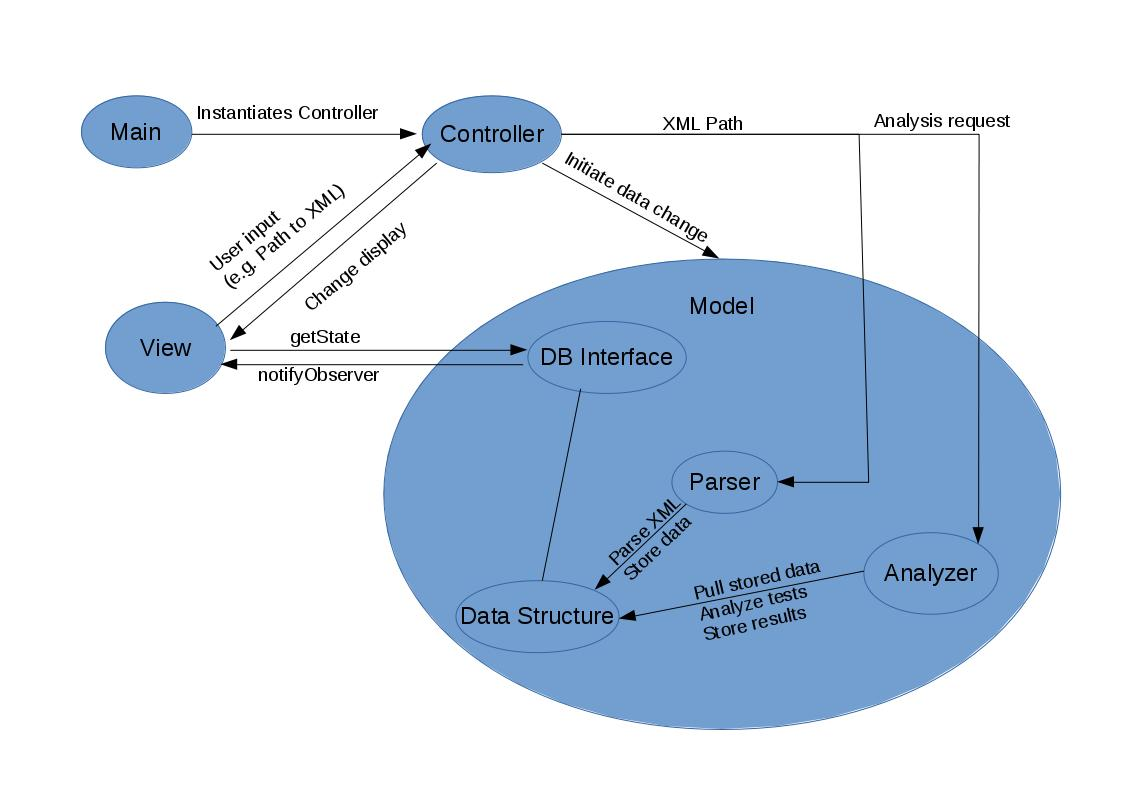
\includegraphics[scale=0.3]{pics/Architecture_diagram.jpg}
\caption{High level architecture} 
\label{HLA}
\end{center}
\end{figure}

In the next step we constructed a central glossary to minimize misunderstandings in our communication and make sure to understand the language of the client. \\ 

\begin{table}[h]
  \caption{Glossary}
  \label{Glossary}
  \centering
  \begin{tabular}{p{2.3cm}||p{10cm}|}
  	Term & Meaning \\ 
  	\hline
  	\hline
  	Test run & A collection of unit tests of one specific build \\ 
  	\hline
  	Failure percentage & Failure percentage of class C = (Number of failed unit tests for class C) / (Total number of unit tests for class C) \\ 
  	\hline
  	TDA & Test Data Analyser (the program to be developed) \\ 
  	\hline
  	Problematic class & Class with a high test failure percentage \\ 
  	\hline
  \end{tabular}
\end{table}

The last task of sprint 0 was to conduct a risk analysis. Most likely we have to deal with sickness of individual persons every now and then. We try to limit the impact of this by good group communication, shared responsibilities and documentation. Also it is likely that the client changes the specifications along the way, what we’re going to cope by building adaptable software with loose coupling and high cohesion. The risks with the highest impact would be someone leaving the project or the complete loss of all our data. We are going to deal with this with shared responsibilities and backups, respectively. A complete and detailed risk analysis is shown in table \ref{Risks}. \\ 

\begin{table}[h]
  \caption{Risk analysis}
  \label{Risks}
  \centering
  \begin{tabular}{p{3cm}||p{5cm}|p{2cm}|p{2cm}|}
  	Risk & Coping & Likelyhood & Impact \\ 
  	\hline
  	\hline
  	Someone leaves the project & Shared Responsibilities & <10\% & Severe \\ 
  	\hline
  	Complete data loss & Back ups & 5\% & Severe \\ 
  	\hline
  	Usage of prohibited packages & Regular checks, test on external IDE & 10\% & High \\ 
  	\hline
  	Sick team member & Shared responsibility, documentation & 50\% & Medium \\ 
  	\hline
  	Client changes specifications & Adaptable software (loose coupling \& high cohesion & 50\% & Medium \\
  	\hline
  	Unprecise specification (missing examples) & Communication with client & 20\% & Medium \\ 
  	\hline
  	Research stories far more complex than expected & Do research early, conservative planning & 5\% & Medium \\ 
  	\hline
  	Differing visions (unnecessary development) & Refular internal communication & 30\% & Medium \\ 
  	\hline
  	Lab PCs insufficient for testing/development & Write performant code & 5\% & Low \\ 
  	\hline
  \end{tabular}
\end{table}